% The figure of the Spark SQL components (fig:sparkArq), in layers: the APIs and
% interfaces; Spark SQL with the DataFrame, SQL and streaming queries, the
% Catalyst optimizer and Adaptive Query Execution; the Tungsten execution engine;
% Spark Core with the distributed execution engine and the cluster managers; and
% the deployment and storage systems, beside the data sources and the other
% components. The style follows the figure of fig:sparkApplicactions
% (figs/chap8/sparkApplicactions.tex of the book). Every box that holds others
% carries its name in bold at its top, and each box is sized to its text, so
% that the figure, printed at the text width, keeps its text as large as it
% can. pdflatex writes sparkArq.pdf.
\documentclass[tikz,border=2pt]{standalone}
\usepackage[T1]{fontenc}
\usepackage{lmodern}
\usetikzlibrary{arrows.meta,positioning,calc,fit,backgrounds}
% A box from its corners (x1,y1) and (x2,y2) in points, y downwards
\newcommand{\bx}[7][]{\node[#1,minimum width={((#5)-(#3))*1pt},
  minimum height={((#6)-(#4))*1pt}] (#2)
  at ({((#3)+(#5))/2*1pt},{-((#4)+(#6))/2*1pt}) {#7};}
\newcommand{\at}[2]{({(#1)*1pt},{-(#2)*1pt})}
\begin{document}
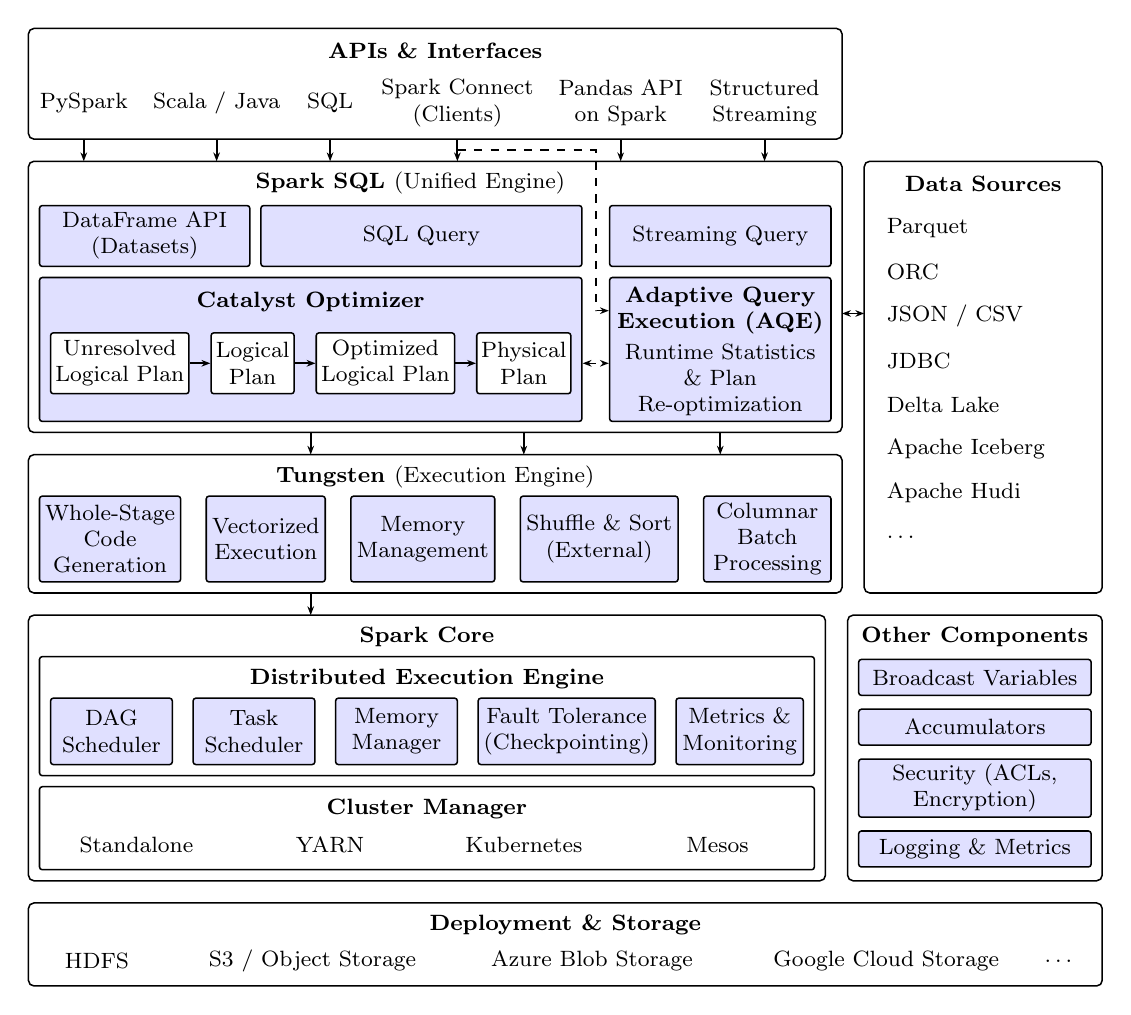
\begin{tikzpicture}[
    every node/.style={font=\footnotesize},
    >={Stealth[length=3.2pt,width=2.4pt]},
    comp/.style={rectangle,rounded corners=1pt,draw,line width=0.55pt,
      fill=blue!12,align=center,inner sep=1pt},
    ext/.style={rectangle,rounded corners=1pt,draw,line width=0.55pt,
      fill=white,align=center,inner sep=1pt},
    layer/.style={rectangle,rounded corners=2pt,draw,line width=0.55pt,
      fill=white},
    lname/.style={align=center,inner sep=1pt},
    title/.style={font=\footnotesize\bfseries,align=center,inner sep=1pt},
    flow/.style={->,line width=0.7pt},
    dflow/.style={->,line width=0.55pt,dashed},
  ]
  % ==================== APIs and interfaces ====================
  \draw[layer] \at{0}{0} rectangle \at{294}{40};
  \node[title] at \at{147}{8} {APIs \& Interfaces};
  \foreach \x/\t in {20/PySpark,68/{Scala / Java},109/SQL,
      155/{Spark Connect\\(Clients)},214/{Pandas API\\on Spark},
      266/{Structured\\Streaming}} {
    \node[lname] at \at{\x}{27} {\t};
    \draw[flow] \at{\x}{40} -- \at{\x}{48};
  }

  % ==================== Spark SQL ====================
  \draw[layer] \at{0}{48} rectangle \at{294}{146};
  \node[title] at \at{138}{56} {Spark SQL \textmd{(Unified Engine)}};
  \bx[comp]{dfapi}{4}{64}{80}{86}{DataFrame API\\(Datasets)}
  \bx[comp]{sqlq}{84}{64}{200}{86}{SQL Query}
  \bx[comp]{strq}{210}{64}{290}{86}{Streaming Query}
  \bx[comp]{cat}{4}{90}{200}{142}{}
  \node[title] at \at{102}{99} {Catalyst Optimizer};
  \bx[ext]{p1}{8}{110}{58}{132}{Unresolved\\Logical Plan}
  \bx[ext]{p2}{66}{110}{96}{132}{Logical\\Plan}
  \bx[ext]{p3}{104}{110}{154}{132}{Optimized\\Logical Plan}
  \bx[ext]{p4}{162}{110}{196}{132}{Physical\\Plan}
  \draw[flow] (p1) -- (p2);
  \draw[flow] (p2) -- (p3);
  \draw[flow] (p3) -- (p4);
  \bx[comp]{aqe}{210}{90}{290}{142}{}
  \node[title] at \at{250}{102} {Adaptive Query\\Execution (AQE)};
  \node[lname] at \at{250}{127} {Runtime Statistics\\\& Plan\\
    Re-optimization};
  \draw[dflow,<->] (p4.east -| cat.east) -- (p4.east -| aqe.west);
  \draw[dflow] \at{155}{44} -- \at{205}{44} -- \at{205}{102} --
    (aqe.west |- 0,-102pt);

  % ==================== Tungsten ====================
  \foreach \x in {102,179,250}
    \draw[flow] \at{\x}{146} -- \at{\x}{154};
  \draw[layer] \at{0}{154} rectangle \at{294}{204};
  \node[title] at \at{147}{162} {Tungsten \textmd{(Execution Engine)}};
  \bx[comp]{t1}{4}{169}{55}{200}{Whole-Stage\\Code\\Generation}
  \bx[comp]{t2}{64.25}{169}{107.25}{200}{Vectorized\\Execution}
  \bx[comp]{t3}{116.5}{169}{168.5}{200}{Memory\\Management}
  \bx[comp]{t4}{177.75}{169}{234.75}{200}{Shuffle \& Sort\\(External)}
  \bx[comp]{t5}{244}{169}{290}{200}{Columnar\\Batch\\Processing}

  % ==================== Spark Core ====================
  \draw[flow] \at{102}{204} -- \at{102}{212};
  \draw[layer] \at{0}{212} rectangle \at{288}{308};
  \node[title] at \at{144}{220} {Spark Core};
  \bx[ext]{dee}{4}{227}{284}{270}{}
  \node[title] at \at{144}{235} {Distributed Execution Engine};
  \bx[comp]{c1}{8}{242}{52}{266}{DAG\\Scheduler}
  \bx[comp]{c2}{59.5}{242}{103.5}{266}{Task\\Scheduler}
  \bx[comp]{c3}{111}{242}{155}{266}{Memory\\Manager}
  \bx[comp]{c4}{162.5}{242}{226.5}{266}{Fault Tolerance\\(Checkpointing)}
  \bx[comp]{c5}{234}{242}{280}{266}{Metrics \&\\Monitoring}
  \bx[ext]{cm}{4}{274}{284}{304}{}
  \node[title] at \at{144}{282} {Cluster Manager};
  \foreach \x/\t in {39/Standalone,109/YARN,179/Kubernetes,249/Mesos}
    \node[lname] at \at{\x}{295} {\t};

  % ==================== Data sources ====================
  \draw[layer] \at{302}{48} rectangle \at{388}{204};
  \node[title] at \at{345}{56} {Data Sources};
  \foreach \y/\t in {72/Parquet,88/ORC,104/{JSON / CSV},120/JDBC,
      136/Delta Lake,152/Apache Iceberg,168/Apache Hudi,184/\dots}
    \node[anchor=west,inner sep=0pt] at \at{310}{\y} {\t};
  \draw[flow,<->] \at{294}{103} -- \at{302}{103};

  % ==================== Other components ====================
  \draw[layer] \at{296}{212} rectangle \at{388}{308};
  \node[title] at \at{342}{220} {Other Components};
  \bx[comp]{o1}{300}{228}{384}{241}{Broadcast Variables}
  \bx[comp]{o2}{300}{246}{384}{259}{Accumulators}
  \bx[comp]{o3}{300}{264}{384}{285}{Security (ACLs,\\Encryption)}
  \bx[comp]{o4}{300}{290}{384}{303}{Logging \& Metrics}

  % ==================== Deployment and storage ====================
  \draw[layer] \at{0}{316} rectangle \at{388}{346};
  \node[title] at \at{194}{324} {Deployment \& Storage};
  \foreach \x/\t in {13/HDFS,65/{S3 / Object Storage},
      167/{Azure Blob Storage},269/{Google Cloud Storage},367/\dots}
    \node[anchor=west,inner sep=0pt] at \at{\x}{337} {\t};
\end{tikzpicture}
\end{document}
